\chapter{Разработка системы} \label{ch3}

	\section{Разработка API-шлюза}

	\subsection{Разработка модуля авторизации}

	Модуль аутентификации является неотъемлемой частью API-шлюза и выполняет важные функции по обеспечению безопасности, идентификации и контроля доступа пользователей к ресурсам системы. Его основная задача – предоставлять механизм регистрации, аутентификации, управления сессиями и обновления токенов, обеспечивая безопасное взаимодействие между клиентскими приложениями и серверными компонентами. Для того, чтобы мы могли идентифицировать пользователя на серверной стороне, проводить его аутентификацию и валидировать права на модификацию информации о видео, загрузку сегментов видео в соответствующую сессию, то есть проводить авторизацию.

	Кроме того, для того, чтобы API-Шлюз имел хорошую поддержку в будущем и позволял дополнять его различной логикой, необходимо унифицировать процесс авторизации и получения информации.
	
	В качестве основного фреймворка для разработки серверных приложений в среде исполнения Node.js оптимальным решением будет использовать NestJS, так как он базируется на низкоуровневом Express и архитектуре клиентского фреймворка Angular, что делает его достаточно удобным и эффектиным инструментом.

	Одним из наиболее безопасных и масштабируемых способов проводить идентификацию и авторизацию является использование протокола OAuth 2.0.
	Структурно он включает в себя следующие основные компоненты:

	\begin{itemize}[label=$\bullet$]
		\item Ресурсный владелец (Resource Owner) — пользователь, владеющий доступом к защищённому ресурсу;
		\item Клиент (Client) — приложение, запрашивающее доступ к ресурсу от имени пользователя;
		\item Сервис авторизации (Authorization Server) — компонент, выполняющий аутентификацию пользователя и выдающий токены доступа;
		\item Сервис ресурсов (Resource Server) — сервер, на котором хранятся защищённые данные и который предоставляет доступ на основании валидного токена.
	\end{itemize}

	Работа протокола заключается в следующем: клиент перенаправляет пользователя на сервис авторизации, где тот подтверждает согласие на предоставление доступа. После этого сервис авторизации выдает клиенту токен доступа (access token) — временный цифровой ключ, позволяющий обращаться к защищённым ресурсам на сервере ресурсов. Поскольку access token имеет ограниченное время действия, вместе с ним может быть выдан и токен обновления (refresh token) — специальный долгоживущий токен, с помощью которого клиент может получить новый access token без повторного участия пользователя. Таким образом, OAuth 2.0 позволяет безопасно и удобно предоставлять ограниченный по объему и времени доступ к данным, избегая необходимости передачи паролей сторонним приложениям.

	Основное преимущество OAuth 2.0 заключается в масштабировании. В текущем проекте в качестве сервера ресурсов выступает рассмотренный API-Шлюз. С использованием этого протокола появляется возможность задействовать разные серверы авторизации для него. В рамках текущего проекта остановимся на одном сервере авторизации, который будет реализован ниже - это вполне соответствует функциональным требованиям системы. Однако при реализации данного протокола необязательно располагать сервис авторизации и сервис ресурсов независимо. Они могут быть частью общего сервиса - API-Шлюза. Это позволит унифицировать процесс авторизации и получения информации об идентифицированном пользователе.
	
	Для реализации модуля необходимо предоставить пользователю возможность проводить регистрацию, аутентификацию и обновление токенов. Так как модуль не представляет какой-то конкретной бизнес логики проекта, его необходимо расположить на отдельном контроллере AuthController - это позволит вынести логику на отдельный слой API.
	
	Для эндпоинтов, которые требуют аутентификации, необходимо реализовать механизм, который бы автоматически её проводил и предоставлял информацию о пользователе из базы данных. Эту логику можно изолировать в декоратор AuthGuard. Логику, связанную непосредственно с генерацией и валидацией JWT токенов, необходимо вынести в отдельный сервис JwtService для соблюдения принципа единственности ответственности. Общую бизнес-логику AuthController и AuthGuard необходимо вынести в общий сервис AuthService для избежания повторения кода.

	Представим взаимодействие между описанными выше классами в виде UML-диаграммы для наглядности. Схема UML модуля авторизации представлена на рисунке \ref{fig:uml_auth}.

	\begin{figure}[ht!] 
		\center
		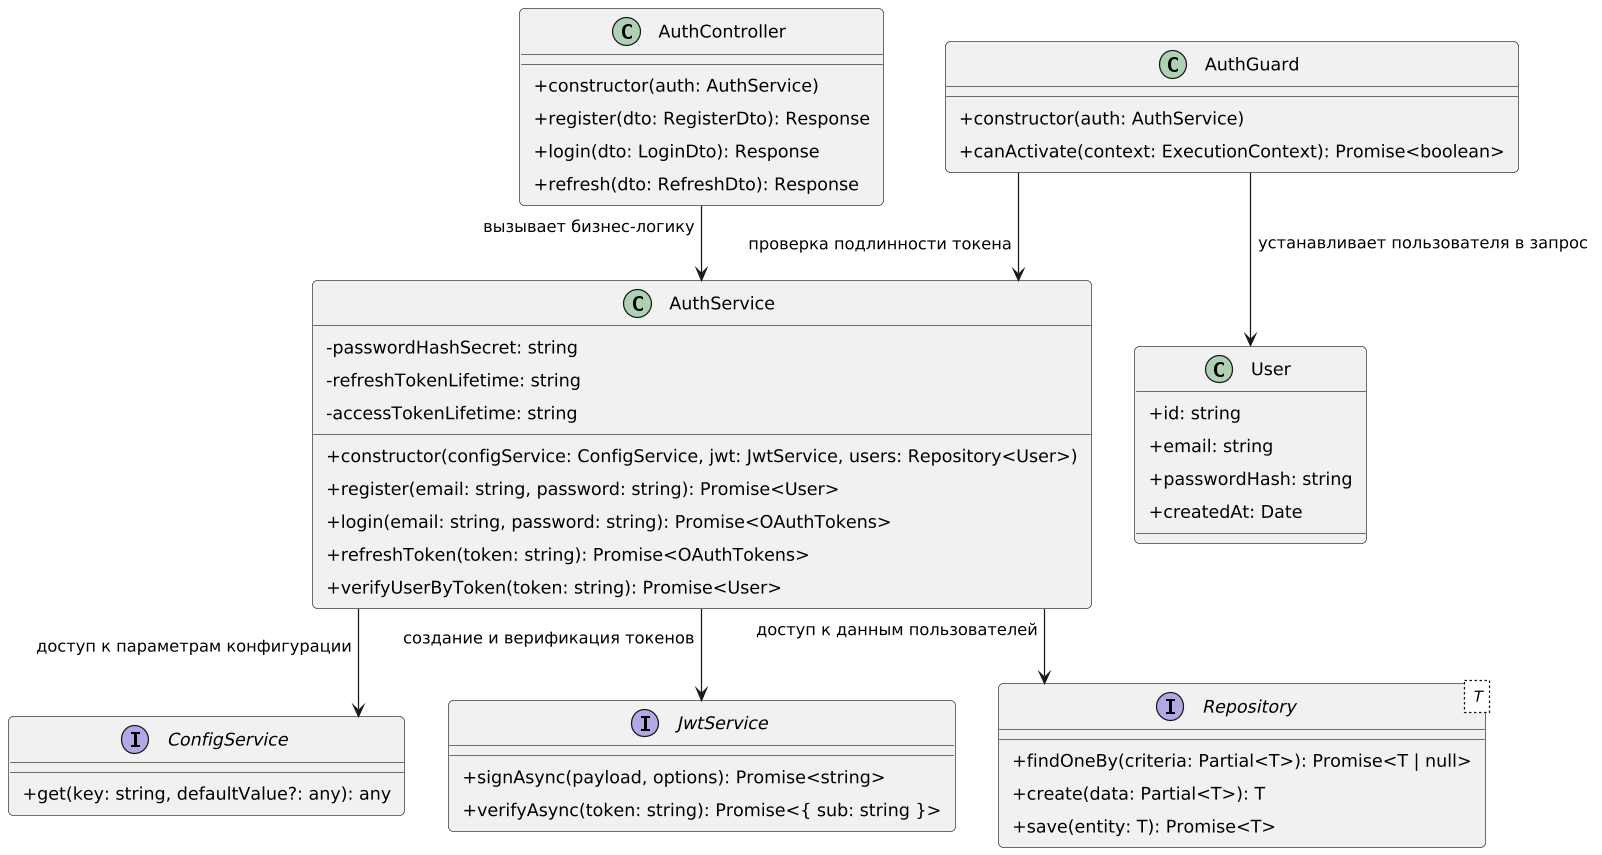
\includegraphics [scale=0.2] {my_folder/images//uml_auth}
		\caption{UML-диаграмма модуля авторизации} 
		\label{fig:uml_auth}  
	\end{figure}

	Из диаграммы видно, что мы можем построить граф зависимостей между классами, благодаря описанию их конструкторов. Более того, не содержат дополнительных аргументов для их конфигурации в конструкторах. Вся необходимая конфигурация инкапуслирована в ConfigService. Это значит, что представленные классы имеют чистые зависимости между друг другом. Такая структура позволяет использовать механизм инъекции зависимостей (англ. dependency injection). Такой механизм поддерживается по умолчанию в NestJS, нам лишь необходимо расставить над классами соответствующие декораторы, выполняющие функционал разметки для определения роли класса или метода в NestJS приложении.

	На диаграмме также изображен дополнительные классы ConfigService и Repository. Первый из них представляет собой сервис для централизованного доступа к конфигурационным параметрам. Этот класс представлен в модуле "@nestjs/common". С помощью специальных конфигурационных объектов из этой же библиотеки можно преобразовывать переменные окружения в удобный формат для конкретного приложения, например, преобразовать литерал из цифр в числовой тип данных. Кроме того, NestJS позволяет не задавать переменные окружения непосредственно в операционной системе, а перечислить их в файле .env проекта. Переменные окружения позволяют отделить конфигурационные параметры от исходного кода, что делает приложение более гибким и безопасным. Это упрощает адаптацию приложения к различным средам без изменения кода, что даст нам возможность управлять конфигурацией проекта в дальнейшем при развёртывании системы. А Repository в контексте NestJS и библиотеки TypeORM представляет собой абстракцию для работы с базой данных. Он предоставляет набор методов для выполнения операций с сущностями, таких как создание, поиск, обновление и удаление данных, без необходимости напрямую писать SQL-запросы.

	При регистрации пользователь отправляет email и пароль через POST-запрос на "/auth/register". Контроллер AuthController обрабатывает этот запрос и вызывает метод register сервиса AuthService, который сначала проверяет, существует ли уже пользователь с таким почтовым адресом в базе данных. Если пользователь найден, выбрасывается исключение. В противном случае создается новый пользователь с хэшированным паролем (с использованием HMAC SHA-256 и секретного ключа), и сохраняется в базе данных. Результат регистрации пользователя возвращается пользователю. Все эти процессы представлены на диаграмме последовательности регистрации на рисунке \ref{fig:register_processes}.

	\begin{figure}[ht!] 
		\center
		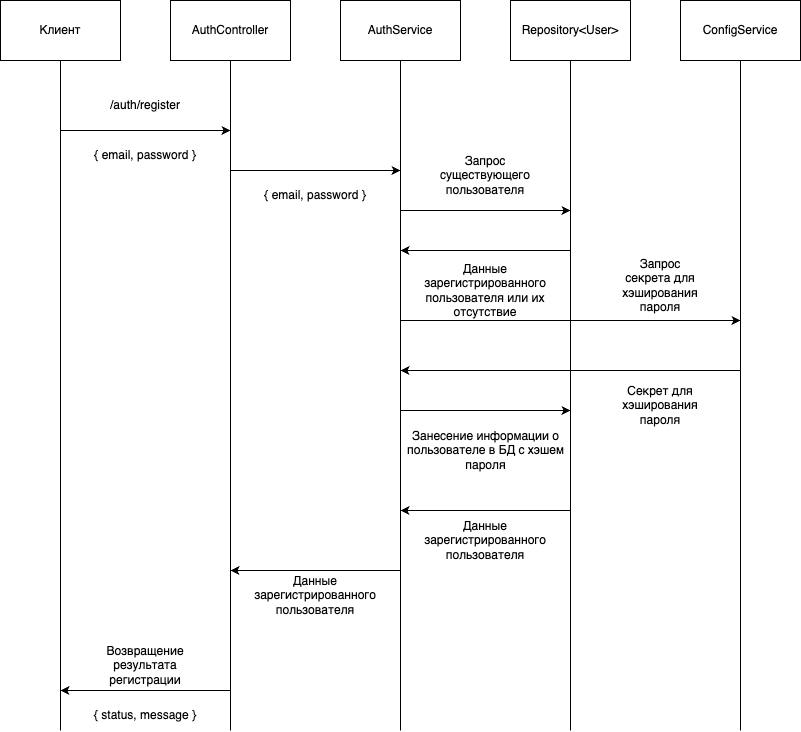
\includegraphics [scale=0.4] {my_folder/images//register_processes}
		\caption{Диаграмма последовательности процессов регистрации пользователя} 
		\label{fig:register_processes}  
	\end{figure}

	Процесс аутентификации пользователя также начинается с запроса с email и паролем на эндпоинт "/auth/login", где контроллер передает данные в сервис аутентификации. Сервис проверяет наличие пользователя в базе данных и сравнивает хэш пароля с сохраненным значением. Перед тем, как генерировать хэш, сервис обращается к ConfigService для получения секрета. Если проверка успешна, генерируются два токена с помощью JwtService: accessToken для доступа к защищенным ресурсам и refreshToken для обновления accessToken по истечении его срока действия. Эти токены возвращаются клиенту, а в случае ошибки отправляется соответствующее сообщение об отказе в доступе. Все описанные процессы выше представлены на диаграмме последовательности аутентификации на рисунке \ref{fig:login_processes}.

	\begin{figure}[ht!] 
		\center
		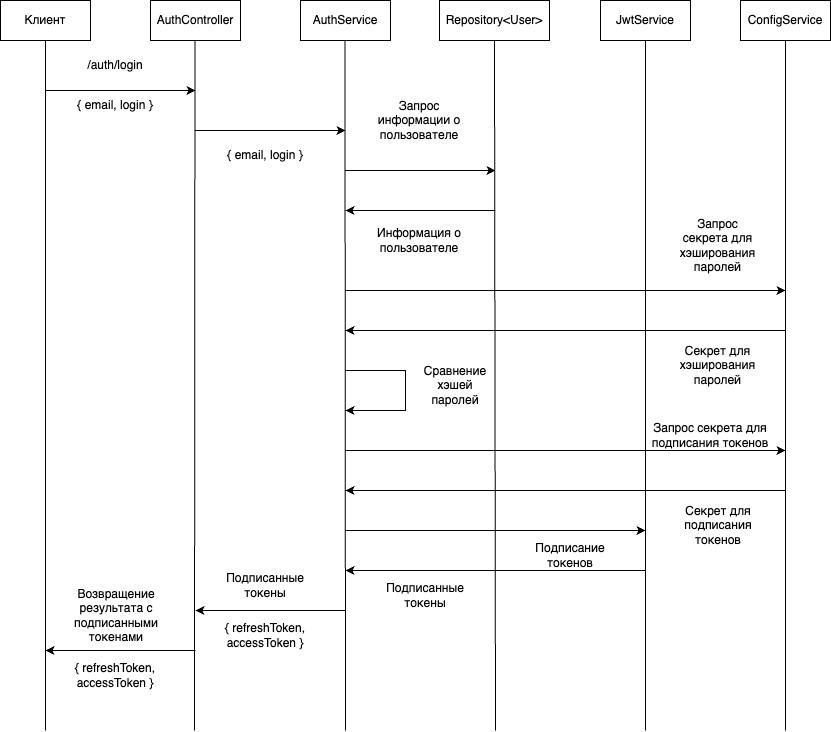
\includegraphics [scale=0.4] {my_folder/images//login_processes}
		\caption{Диаграмма последовательности процессов аутентификации пользователя} 
		\label{fig:login_processes}  
	\end{figure}

	Внешним входом для использования модуля авторизации в других частях API-Шлюза является класс AuthGuard. Другие контроллеры могут его использовать как часть промежуточного слоя обработки HTTP запроса определённых эндпоинтов. Он наследуется от базового механизма защиты NestJS - PassportAuthGuard со стратегией "local". В нём переопределяется метод canActivate и дополняется специфичной логикой проекта. При каждом запросе AuthGuard извлекает заголовок авторизации (Authorization) из входящего HTTP-запроса и проверяет его наличие. Затем с помощью метода verifyUserByToken из AuthService происходит верификация токена, и если пользователь успешно идентифицирован, он добавляется в объект запроса (request.user), что позволяет другим обработчикам эндпоинтов API-Шлюза обращаться к аутентифицированному пользователю. Если токен отсутствует, некорректен или верификация не удалась, выбрасывается исключение UnauthorizedException, которое приводит к возврату ошибки со статусом 401 (Unauthorized).

	\subsection{Разработка головного модуля}

	Головной модуль приложения отвечает за обработку запросов пользователей, связанных с их данными и видеоконтентом. Точкой входа в этот модуль является класс AppController, который содержит набор HTTP-эндпоинтов. В частности, модуль должен содержать логику, которая отвечает за возвращение информации об аутентифицированном пользователе, создание новой записи видео, потоков и инициализации загрузочных сессий для последующей загрузки сегментов видеоконтента, а также в нём должна содержаться логика обработки загрузки сегментов видеоконтента, осуществляя проверку прав доступа и корректности данных, передаваемых пользователем. Кроме того, модуль должен предоставлять возможность для пользователя отслеживать прогресс и статус загрузки потоков видео. Перечисленную выше функциональность можно разделить на следующие эндпоинты:

	\begin{itemize}[label=$\bullet$]
		\item me - получение информации о текущем аутентифицированном пользователе по токену доступа (accessToken);
		\item upload - загрузка сегмента видео для определённой сессии загрузки;
		\item state - получение текущего состояния видео и связанных потоков, сессий загрузки;
		\item create-video - создание видео и связанных потоков, сессий загрузки.
	\end{itemize}

	Все перечисленные выше эндпоинты являются REST и могут использовать JSON формат для взаимодействия между сервером и клиентом, кроме "upload". Этот эндпоинт принимает в качестве тела запроса данные в виде последовательности байт. Он должен быть настроен таким образом, чтобы принимать HTTP-запросы с MIME-type равным "application/octet-stream". Сама разметка сегмента видео должна быть определена в заголовках запроса, что предусматривает их семантика.

	Основная работа головного модуля API-Шлюза заключается в обработке пользовательских запросов, первичной валидации данных полученных от пользователей, а также возврате в безопасном формате данных клиентам. При обработке эндпоинта "me" головной сервис должен вернуть безопасное представление аутентифицированного пользователя или вернуть результат с ошибкой при отсутствии такового. Необходимость в отдельном эндпоинте "me" объясняется тем, что клиентскому приложению в самом начале своего жизненного цикла необходимо определить текущий статус аутентификации пользователя. Это связано со сроком жизни токенов аутентификации - он ограничен. На уровне клиента узнать, просрочен ли тот или иной токен, нет возможности, поэтому необходимо отправить предварительный запрос на сервер.
	
	Вся перечисленная логика выше не может находиться в контроллере AppController, потому что он должен отвечать только за работу с HTTP запросами. Отделение бизнес-логики от контроллера и её вынесение в отдельный класс AppService необходимо для того, чтобы разделить интерфейс взаимодействия с клиентами и непосредственную обработку данных. В AppService следует вынести работу с базой данных с помощью ранее рассмотренных репозиториев TypeORM, логику создания видео, управления потоками и загрузочными сессиями, а также обработку входящих сегментов видеоконтента.
	
	Асинхронную передачу данных, связанную с загрузкой видеофрагментов, логично вынести в отдельный класс ChunkExchangeService, который будет использовать брокер сообщений RabbitMQ для передачи задач на выполнение сервису-загрузчику.
	
	Важно также учитывать, что возвращать информацию, полученную из базы данных, в исходном виде нельзя, так как это не соответствует требованиям безопасности системы. Перед отправлением ответа пользователю данные необходимо предварительно преобразовать. За это будет отвечать VideoConverterService.
	
	UML-диаграмма модуля с учётом разделения бизнес логики на соответствующие классы представлена на рисунке \ref{fig:uml_gateway_main}.

	\begin{figure}[ht!] 
		\center
		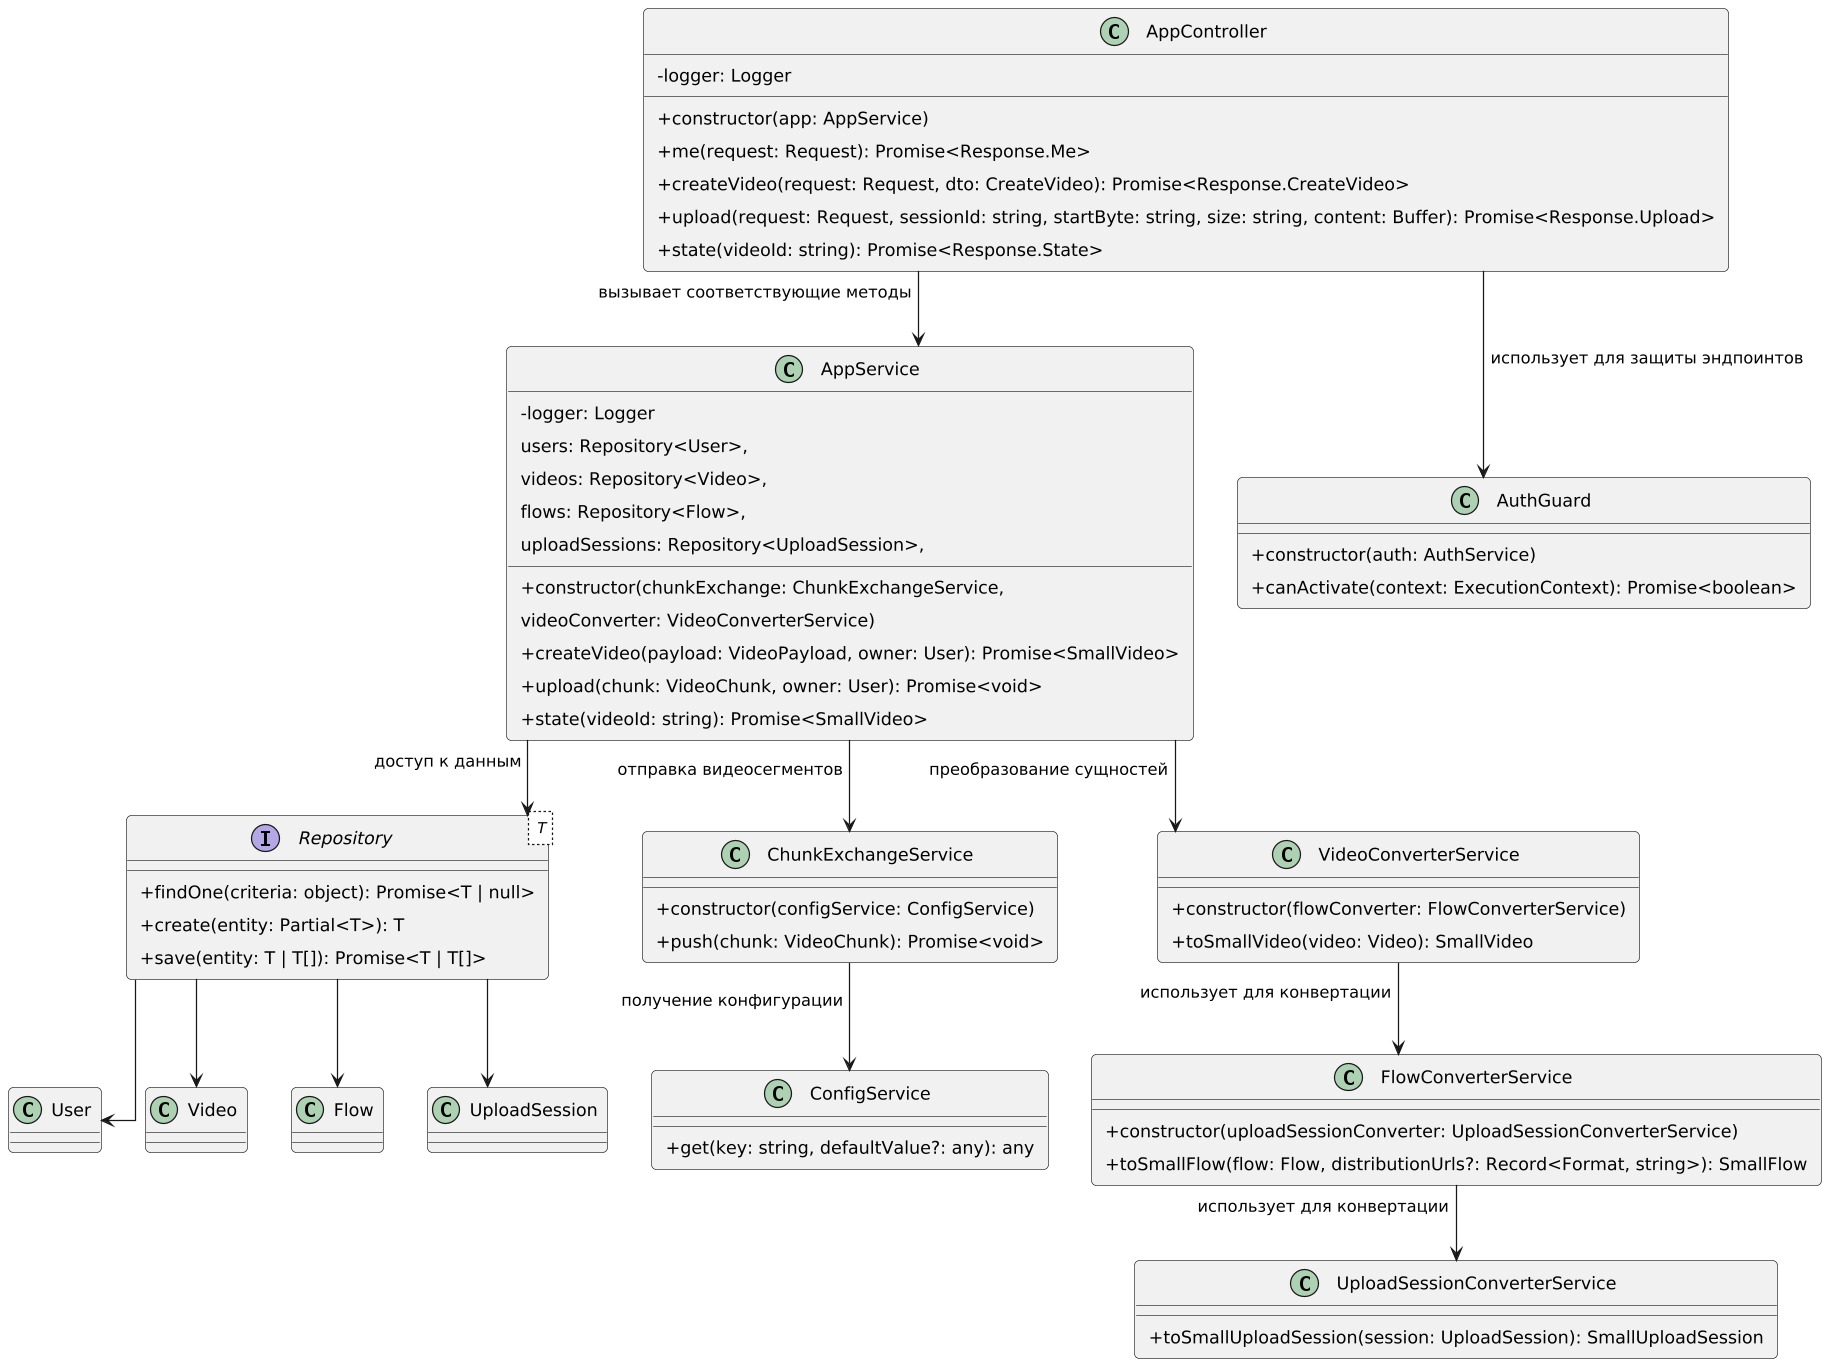
\includegraphics [scale=0.2] {my_folder/images//uml_gateway_main}
		\caption{UML-диаграмма головного модуля API-Шлюза} 
		\label{fig:uml_gateway_main}  
	\end{figure}

	Рассмотрим каждый из эндпоинтов в отдельности ниже.

	Эндпоинт "me" предназначен для получения информации о текущем аутентифицированном пользователе. Он использует защитный механизм AuthGuard, описанный ранее в данной главе, который отвечает за извлечение и верификацию авторизационного токена из запроса. После успешной проверки токена AuthGuard получает экземпляр пользователя из базы данных и прикрепляет его к объекту запроса. Далее в самом эндпоинте происходит конвертация данных пользователя в специальный объект, который содержит только безопасные поля, исключая конфиденциальные данные - хэш пароля, создавая тем самым DTO (Data Transfer Object). Использование AppService здесь не требуется, так как вся бизнес-логика этого эндпоинта уже инкапсулирована в AuthGuard.

	Эндпоинт "create-video" обрабатывает запросы от клиента с телом, содержащим название видео (title), описание (description) и массив размеров потоков видеоконтента (totalBytesList). Он также определяет и количество итоговых потоков, которые будут загружены для этого экземпляра видео. Этот эндпоинт также использует зашитный механизм AuthGuard, соответственно, требует от пользователя токен доступа. После успешной аутентификации экземпляр пользователя извлекается из объекта запроса и передаётся в метод createVideo класса AppService. В этом методе создаётся новая сущность видео, которая сохраняется в базе данных. Затем для каждого элемента списка totalBytesList создаются соответствующие потоки (Flow) и сессии загрузки (UploadSession). Эти сущности также сохраняются в базу данных и связываются с созданным видео. В конце выполнения метода происходит конвертация созданных сущностей в компактный объект (SmallVideo) при помощи VideoConverterService для отправки обратно клиенту. Этот сервис, в свою очередь, инъектирует как зависимость себе FlowConverterService и переводит потоки тоже в безопасные и компактные объекты (SmallFlow). А он, в свою очередь, инъектирует UploadSessionConverterService, который делает то же самое для объекта сессии загрузки. В ответе клиенту возвращается статус выполнения запроса и полученный компактный объект с информацией о созданном видео и его загрузочных потоках в соответствии с их порядком в запросе. Все процессы , описанные выше, представлены на диаграмме последовательности на рисунке \ref{fig:create_video_processes}.

	\begin{figure}[ht!] 
		\center
		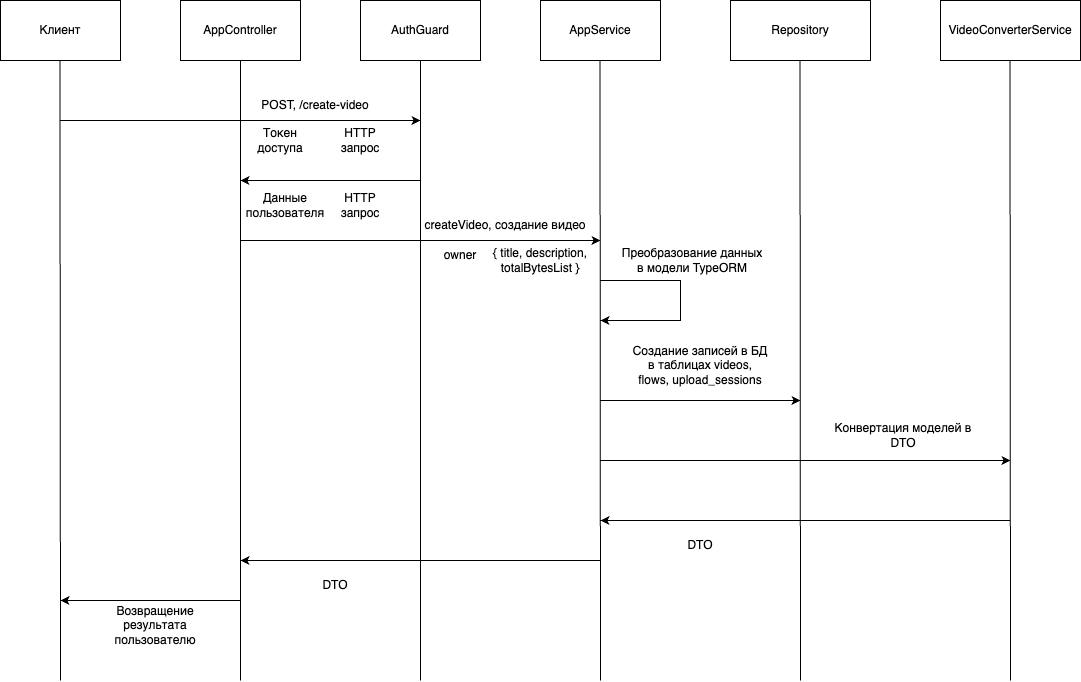
\includegraphics [scale=0.37] {my_folder/images//create_video_processes}
		\caption{UML-диаграмма головного модуля API-Шлюза} 
		\label{fig:create_video_processes}  
	\end{figure}

	Эндпоинт "upload" ожидает от клиента POST-запрос, содержащий идентификатор сессии загрузки (sessionId в URL), номер начального байта (x-start-byte) и размер сегмента (x-size) в заголовках запроса, которые являются разметкой загружаемого сегмента, а также бинарные данные сегмента в теле запроса. Эндпоинт также защищён с помощью механизма авторизации AuthGuard. После проверки авторизации контроллер преобразует заголовки с номером начального байта и размером в числовой формат и проверяет их корректность. Далее данные передаются в метод upload сервиса AppService, который извлекает из базы данных соответствующую сессию загрузки вместе с её связанными объектами видео, потока и пользователя-владельца. Запрос осуществляется с помощью INNER JOIN оператора PgSQL. Затем сервис проверяет права доступа, удостоверяясь, что сессия загрузки принадлежит пользователю, отправившему запрос. В случае успешной проверки чанки отправляются через компонент ChunkExchangeService в брокер сообщений RabbitMQ в соответствующий обменник. По завершении этих действий клиенту возвращается ответ с информацией об успешной загрузке сегмента. Все процессы, описанные выше, представлены на диаграмме последовательности на рисунке \ref{fig:chunk_upload_processes}.

	\begin{figure}[ht!] 
		\center
		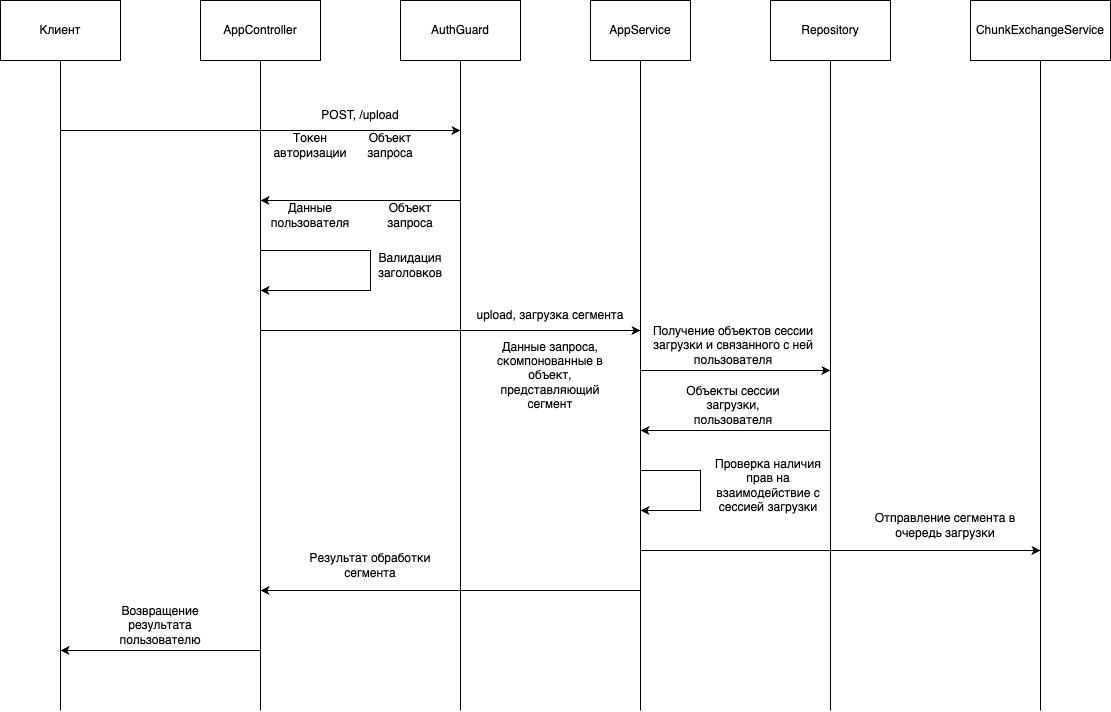
\includegraphics [scale=0.37] {my_folder/images//chunk_upload_processes}
		\caption{Диаграмма последовательности процессов загруки сегмента видео} 
		\label{fig:chunk_upload_processes}  
	\end{figure}

	Процесс передачи сегмента в очередь в ChunkExchangeService тоже можно декомпозировать более детально. Метод push этого класса предназначен для асинхронной передачи сегментов в брокер сообщений RabbitMQ с помощью канала подключения протокола AMQP. Этот метод принимает сформированный объект сегмента видео. В начале метода формируются специальные заголовки сообщения, содержащие необходимую информацию для корректной обработки сегмента на принимающей стороне. После этого сообщение публикуется в соответствующий обменник, параметры которого извлекаются из ConfigService, то есть из соответствующих переменных окружения, что позволяет легко изменять параметры взаимодействия с брокером без модификации кода. Далее метод ожидает подтверждения получения или отказа (ack/nack) от обработчика, после чего разрешает или отклоняет соответствующий асинхронный запрос. Диаграмма последовательности отправки сегмента в очередь сообщений представлена на рисунке \ref{fig:queue_sending_processes}.

	\begin{figure}[ht!] 
		\center
		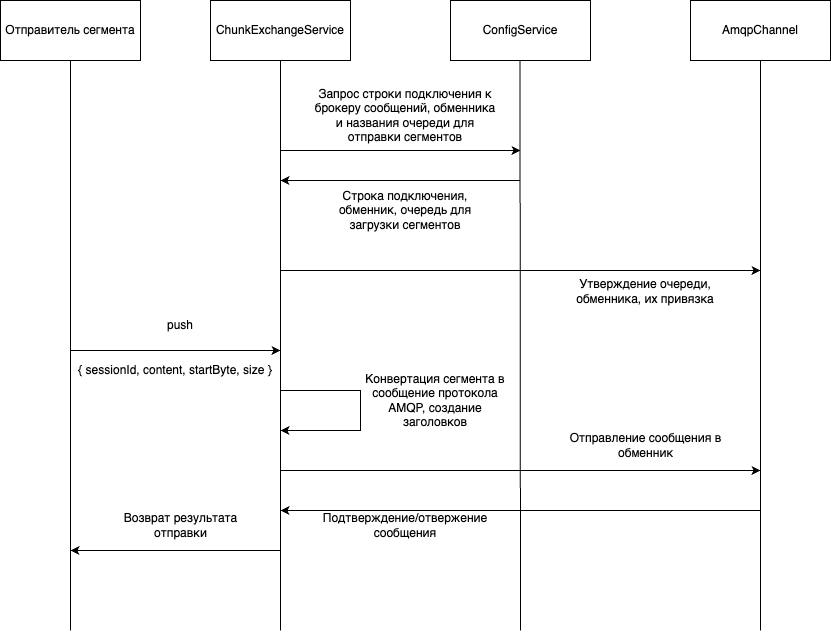
\includegraphics [scale=0.4] {my_folder/images//queue_sending_processes}
		\caption{Диаграмма последовательности отправки сегмента видео в очередь сообщений} 
		\label{fig:queue_sending_processes}  
	\end{figure}

	Эндпоинт "state" ожидает от клиента GET-запрос, содержащий идентификатор видеозаписи (videoId) в URL. Внутри обработчика этого запроса контроллер вызывает метод state класса AppService. Сервис выполняет поиск записи видео в базе данных по указанному идентификатору и дополнительно извлекает связанные с ним потоки и сессии загрузки. Если видеозапись не найдена, сервис генерирует ошибку NotFoundError, которая перехватывается контроллером и преобразуется в HTTP-ответ с соответствующим статусом ошибки. Если же запись видео успешно найдена, она конвертируется в компактный формат (SmallVideo) с помощью сервиса VideoConverterService и отправляется обратно клиенту.

	\section{Разработка сервиса-хранилища статического видеоконтента}

	Видео для адаптивного стриминга с использованием протоколов HLS и DASH представлено в виде соответствующих манифестов .m3u8 и .mpd и связанных с ними файлов-чанков формата MPEG-TS и M4S, описывающих последовательность сегментов и параметры поиска. Такая структура позволяет сохранять и передавать неизменяемые файлы непосредственно через специализированный сервер. Сохранение данных в файловой системе обеспечит высокую скорость доступа к манифестам и чанкам видеоконтента, а HTTP-сервер, отвечающий за их раздачу, позволит браузерам кэшировать получаемые ресурсы.

	Таким образом, этот сервис разделяется на два независимых модуля: UploadModule - модуль загрузки, DistributionModule - модуль раздачи. Оба модуля имеют общий ресурс в виде файловой системы, где статические данные будут храниться. Это означает, что путь к директории в файловой системе, где будут храниться данные, необходимо вынести в отдельную переменную окружения - ROOT\_PATH, которую будут использовать оба модуля. Несмотря на это, у каждого модуля будет использоваться свой экземпляр ConfigService, так как настройки каждого из них специфичны.

	Как ранее отмечалось, для межсерверной передачи файлов оптимальным способом является использование FTP протокола. Соответственно, модуль загрузки должен поддерживать FTP сервер, который готов обрабатывать операции взаимодействия с файлами. Node.js библиотека "ftp-srv" с корневым классом FtpSrv поддерживает эту возможность. Этот протокол по умолчанию раздаёт порт 20 для установления управляющего соединения. Этот порт достаточно легко вынести в переменную окружения для конфигурации. Однако протокол также динамически может использовать порты для свободных подключений в диапазоне от 1024 до 65535. Этот диапазон необходимо также сконфигурировать и ограничить, чтобы сделать работу сервиса более предсказуемым, конфигурируемым и надёжным.

	Для модуля с раздачей статики необходимо учитывать только путь до корневой директории, где хранятся файлы, а также порт HTTP-сервера. Для запуска сервера с раздачей статического контента оптимальным решением будет использовать модуль ServeStaticModule, который поставляется из фреймворка NestJS, для беспрепятственной интеграции со средой. При определении DistributionModule описанный выше модуль необходимо передать в массив значений imports в объект декоратора Module для его инициализации. Важно также учесть и политики безопасности сервиса. Он должен возвращать HTTP ответ только разрешённым источникам, в текущем проекте - только плееру. Для этого также необходимо определить переменную окружения - PLAYER\_ORIGIN.
	Кроме того, также необходимо правильно настроить процесс загрузки двух модулей в одном проекте, так как модуль загрузки не должен раздавать никаких дополнительных портов, кроме системных для FTP. Для этого при инициализации модуля с помощью NestFactory будем использовать createApplicationContext вместо метода create, как для обычных HTTP приложений. Программный код старта приложения с учетом требований представлен ниже.

	\begin{lstlisting}[caption=Код старта сервиса-хранилища]
		async function bootstrap() {
			const [distribution] = await Promise.all([
			NestFactory.create(DistributionModule),
			NestFactory.createApplicationContext(UploadModule),
			]);
			
			distribution.enableCors({
				origin: [
				PLAYER_ORIGIN,
				],
				methods: [
				'GET',
				],
			});
			
			await distribution.listen(process.env.DISTRIBUTION_PORT ?? 4050);
		}
		
		bootstrap();
	\end{lstlisting}

	UML-диаграмма сервиса с учётом требований выше представлена на рисунке \ref{fig:uml_holder}.

	\begin{figure}[ht!] 
		\center
		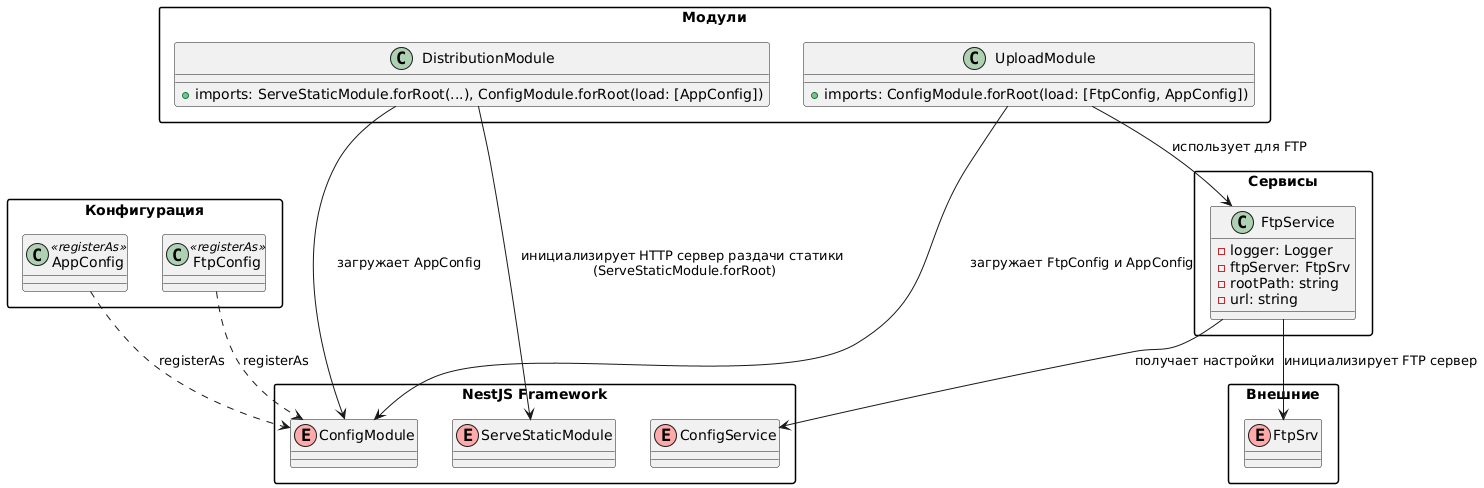
\includegraphics [scale=0.33] {my_folder/images//uml_holder}
		\caption{UML-диаграмма сервиса-хранилища статического видеоконтента} 
		\label{fig:uml_holder}  
	\end{figure}
	
	\section{Разработка сервиса-транскодировщика}

	Перед тем, как загрузить статический видеоконтент на сервис-хранилище, его необходимо транскодировать в необходимые видео и аудио кодеки и преобразовать в форматы DASH и HLS. Это является основной зоной ответственности этого сервиса. Важно также учитывать, что сервис, являясь частью системы, должен предоставлять интерфейсы для взаимодействия с другими сервисами, а также поддерживать протоколы других связанных компонентов. Это фактически означает, что сервис должен предоставлять HTTP-эндпоинты для сервиса-загрузчика, а также поддерживать FTP-клиент для передачи сформированного контента из файлов на сервис-хранилище. Последнее требование говорит о том, что сформированные файлы должны сохраняться либо с помощью абстракции, которая умеет представлять псевдо-файловую систему в оперативной памяти, либо непосредственно в файловой системе.

	Как было отмечено ранее, в этом сервисе будет использоваться продукт с открытым исходным кодом - FFmpeg. Он представлен в виде набора библиотек, в том числе и программы-кодировщики, и консольных утилит. Использование этого программного осуществляется с помощью создания процесса "ffmpeg" с соответствующим набором параметров, который будет рассмотрен далее. Это означает, что каждый такой процесс будет привязан к процессу-родителю и необходимо предусмотреть механизм маршрутизации к конкретной реплике сервиса.

	Все конфигурируемые параметры необходимо вынести в переменные окружения для гибкости настройки этого сервиса.
	Точкой входа в сервис будет являться контроллер AppController. Он принимает HTTP-запросы, передаёт на выполнение главному сервису AppService и возвращает результат пользователю в определённом формате. Контроллер инъектирует в конструктор два сервиса: AppService - содержит методы, реализующие бизнес-логику работы с потоками FFmpeg, файловой системой и FTP клиентом, ConfigService - инкапсулирует работу с конфигурацией сервиса. Из конфигурации контроллер извлекает с помощью метода get извлекаются следующие параметры: globalPrefix - глобальный URL-префикс для API для текущей реплики, а также host - хост, на котором развернут текущий сервис для внешнего клиента (сервиса-загрузчика).
	
	Рассмотрим реализацию каждого эндпоинта в отдельности ниже:
	
	\begin{itemize}[label=$\bullet$]
		\item createFlow: принимает запрос, извлекает из его параметров uploadSessionId, логирует идентификатор новой сессии для отладки работы сервиса при развертывании, вызывает метод createFlow экземпляра AppService с полученным идентификатором сессии загрузки, использует конфигурационные параметры globalPrefix и host, чтобы динамически сформировать часть URL маршрутизации к текущей реплике, и возвращает его пользователю. Пример сформированного URL: "http://fflow:4050/r1";
		\item deleteFlow: принимает запрос, извлекает из его параметров uploadSessionId, вызывает одноимённый метод экземпляра AppService и передаёт в него идентификатор сервиса загрузки. Обрабатывает ошибку FlowNotFoundError и возвращает 404 код состояния пользователю, если поток не найден;
		\item pushToFlow: принимает в качестве тела запроса бинарные данные видео, логирует идентификатор сессии и размер полученных данных для отладки в будущем, вызывает одноименный метод объекта AppService для передачи данных по входящий поток FFmpeg. Как и эндпоинт выше, возвращает 404 код состояния в случае отсутствия созданного потока;
		\item finishFlow: принимает запрос на завершение текущего процесса, извлекает параметр uploadSessionId, вызывает одноимённый метод экземпляра AppService. В случае, если поток не найден, возвращает пользователю 404 код состояния.
	\end{itemize}

	Однако фактическое добавление globalPrefix для текущей реплики надо дополнительно настроить. NestJS содержит реализованный промежуточный слой, который устанавливает всему приложению глобальный префикс - setGlobalPrefix. Запросы на создание потока в реплику будут приходить без этого префикса, так как он будет распределяться равномерно между созданными репликами с помощью балансировщика нагрузки. Чтобы разрешить эту проблему конфигурации, необходимо написать промежуточный слой обработки запрашиваемого URL. Если URL запроса не будет начинаться с глобального префикса, он будет добавлен принудительно, чтобы мы могли обработать запросы без конкретной маршрутизации. Кроме того, код инициализации также должен обрабатывать запросы с телом в виде бинарных данных. Для этого при инициализации необходимо задать промежуточный слой, который бы обрабатывал запросы с заголовком "Content-Type": "application/octet-stream". Код инициализации приложения с учётом требований выше представлен ниже:

	\begin{lstlisting}[caption=Код старта сервиса-траскодировщика]
		function globalPrefixFiller(globalPrefix: string = '') {
			return (req, res, next) => {
				if (!req.url.startsWith(globalPrefix)) {
					req.url = globalPrefix + req.url;
				}
				next();
			};
		}
		
		async function bootstrap() {
			const app = await NestFactory.create(AppModule);
			
			app.use(bodyParser.raw({ type: 'application/octet-stream', limit: '10mb' }));
			app.setGlobalPrefix(process.env.GLOBAL_PREFIX);
			app.use(globalPrefixFiller(process.env.GLOBAL_PREFIX));
			
			await app.listen(process.env.PORT ?? 5050);
		}
		
		bootstrap();
	\end{lstlisting}

	Перед описанием главного сервиса AppService рассмотрим компоненты, от которых он зависит.

	Для того, чтобы файлы, созданные с помощью FFmpeg, отправлялись на сервис-хранилище, необходимо реализовать FTP клиент. Основные операции и подключение к FTP серверу реализуются в библиотеке “basic-ftp” - она является единственным поддерживаемым FTP клиентом на Node.js с открытым исходным кодом на текущий момент. Для передачи файлов с помощью этого протокола необходимо каждый раз создавать новую FTP сессию, так как каждая из них содержит свой контекст. Эту логику необходимо выделить в отдельный класс FtpSession. Он содержит два поля: client - экземпляр FTP клиента из библиотеки “basic-ftp”, options - настройки подключения к FTP. А также методы: асинхронный launch - выполняет подключение к серверу, createDir - создаёт директорию на сервере по указанному пути, uploadFromDir - загружает содержимое локальной директории на FTP сервер, destroy - закрывает FTP соединение и освобождает ресурсы. Однако, чтобы напрямую не создавать FTP сессии каждый раз при использовании, так как параметры подключения будут достаточно типовыми и конфигурируемыми, логику их инициализации можно вынести в отдельный класс FtpSessionsOrchestratorService. Этот класс внедряет сервис конфигурации ConfigService и получает из него параметры подключения к FTP-серверу: хост и порт (с возможностью задать значения по умолчанию). Он имеет единственный метод create, который создаёт и запускает новую FTP-сессию, возвращая её экземпляр.

	Работу с потоками FFmpeg сервисам вынесем в отдельный сервис - FFlowService. В конструкторе происходит инициализация конфигурационных параметров из ConfigService. Конструктор FFlowService инициализирует следующие параметры из сервиса конфигурации:

	\begin{itemize}[label=$\bullet$]
		\item videoCodec — кодек для видео (по умолчанию 'libx264');
		\item audioCodec — кодек для аудио (по умолчанию 'aac');
		\item videoBitrate — битрейт видео (по умолчанию '5000k');
		\item audioBitrate — битрейт аудио (по умолчанию '192k');
		\item dashSegmentDuration — длительность сегмента для DASH (в секундах, по умолчанию 10);
		\item dashSegmentFormat — формат сегмента для DASH (по умолчанию 'mp4');
		\item hlsTime — длительность сегмента для HLS (в секундах, по умолчанию 4);
		\item hlsPlaylistType — тип плейлиста HLS (по умолчанию 'vod');
		\item logLevel — уровень логирования FFmpeg (по умолчанию 'debug').
	\end{itemize}

	В качестве кодеков будут использоваться H.264 и AAC, как было определено в первой главе. Также в конструкторе инициализируется in-memory хранилище flowBySessionId, представляющее собой словарь, в котором ключом является идентификатор сессии (uploadSessionId), а значением — экземпляр дочернего процесса (ChildProcess), связанный с конкретным процессом FFmpeg.

	Класс выше также содержит следующие методы:

	\begin{itemize}[label=$\bullet$]
		\item createFlow: формирует аргументы командной строки для FFmpeg с использованием билдера ffmpegArgsBuilder, включая входной поток (pipe:0) и два выходных — для DASH и HLS. Благодаря выделенному входному потоку процессы FFmpeg могут существовать без ограничений по времени и принимать бинарные данные асинхронно. Если для указанного uploadSessionId уже существует активный процесс, выбрасывается исключение FlowAlreadyExistsError. После успешного создания дочернего процесса FFmpeg, он сохраняется в flowBySessionId;
		\item deleteFlow: завершает активный процесс FFmpeg с помощью метода killFlow. После завершения процесс удаляется из словаря. Метод предполагает дальнейшее \item расширение с очисткой временных ресурсов;
		\item pushToFlow: записывает переданный бинарный буфер в stdin процесса FFmpeg. Если поток не существует, выбрасывается FlowNotFoundError;
		\item finishFlow: завершает поток корректно, закрывая stdin процесса и ожидая завершения выполнения через listenDestroy. После завершения процесса он удаляется из словаря flowBySessionId;
		\item killFlow: является низкоуровневым методом для принудительного завершения процесса с помощью SIGKILL. Аналогично finishFlow, он дожидается завершения и очищает записи из внутреннего хранилища;
		\item listenDestroy: подписывается на события exit и close дочернего процесса.
	\end{itemize}

	Главный сервис AppService в конструкторе из ConfigService извлекает имя выходного манифеста, на основе которого формируются конечные имена DASH и HLS файлов (manifest.mpd, manifest.m3u8). Этот сервис инъектирует в конструкторе следующие зависимости: ранее рассмотренные FFlowService и FtpSessionsOrchestratorService. AppService содержит следующие методы:

	\begin{itemize}[label=$\bullet$]
		\item createFlow: подготавливает пути директорий вывода (для DASH и HLS) и создает параметры для процесс FFmpeg, указав соответствующие пути вывода, кодеки и остальные перечисленные ранее настройки. После этого FFlowService запускает процесс FFmpeg с заданными параметрами вывода;
		\item deleteFlow: завершает активный процесс FFmpeg, связанный с сессией, и удаляет все временные файлы и директории, связанные с этой сессией из файловой системы;
		\item finishFlow: завершает поток транскодирования через FFlowService, после чего инициирует FTP-сессию через FtpSessionsOrchestratorService, создает директорию на удалённом сервере и загружает туда все сгенерированные файлы из локальной директории сессии. После успешной отправки файлов происходит очистка локального каталога и завершение FTP-сессии;
		\item pushToFlow: передаёт бинарные данные в stdin активного FFmpeg-процесса, делегируя эту задачу FFlowService.
	\end{itemize}

	Для визуализации структуры сервиса была построена UML-диаграмма классов, представленная на рисунке \ref{fig:uml_fflow}.

	\begin{figure}[ht!] 
		\center
		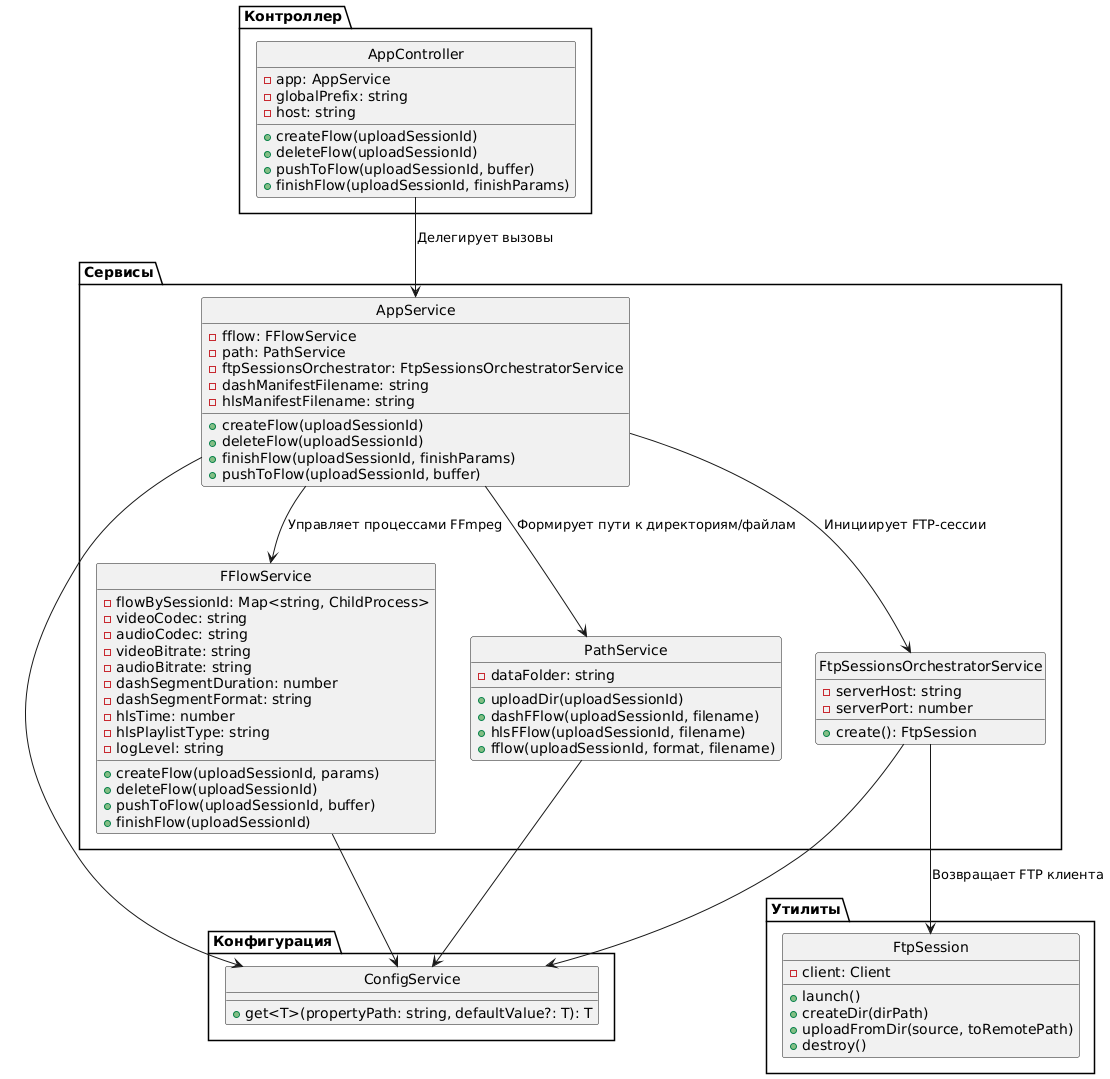
\includegraphics [scale=0.37] {my_folder/images//uml_fflow}
		\caption{UML-диаграмма сервиса-транскодировщика} 
		\label{fig:uml_fflow}  
	\end{figure}

	\section{Разработка сервиса-загрузчика}
	
	Между сервисом-транскодировщиком и API-Шлюзом располагается промежуточный сервис, который занимается выполнением задач по валдиации и обработке видеосегментов, актуализацией состояния видео, потоков и сессий загрузки, а также удалением просроченных видео и их ресурсов. Вся перечисленная выше логика входит в зону ответственности сервиса-загрузчика.

	\subsection{Разработка потребителя задач обработки сегментов}
	
	Как было указано ранее, API-Шлюз взаимодействует с сервисом-загрузчиком с помощью очереди RabbitMQ, передавая в неё задачи для обработки видеосегментов, а фактически - сегменты с разметкой в виде заголовков и меткой сообщения.

	Для того чтобы считывать данные из очереди RabbitMQ, необходимо выделить логику, связанную с обработкой событий очереди, в отдельный класс — ChunkConsumerService. Этот класс ответственен за асинхронное получение сообщений из очереди, их валидацию и передачу на дальнейшую обработку.

	В качестве фреймворка для реализации сервиса загрузчика был выбран Spring Boot на язык программирования Java. Он также, как и NestJS, поддерживает механизм инъекции зависимостей, поэтому мы можем строить зависимости между компонентами сервиса, проставляя соответствующие аннотации.

	Для того чтобы считывать данные из очереди RabbitMQ, необходимо выделить логику, связанную с обработкой событий очереди, в отдельный класс - ChunkConsumerService. За инициализацию подключения к очереди отвечает ChunkQueueConfiguration, который содержит создание фабрики экземпляров Connection и Channel. В классе ChunkConsumerService реализован метод init, помеченный аннотацией @PostConstruct, который выполняется после инициализации объекта. В этом методе осуществляется пассивная декларация очередей (uploadQueue и replyQueue), так как за их создание отвечает головной сервис API-Шлюз. После этого инициализируется обработчик сообщений через метод basicConsume класса, который принимает два обработчика сообщений — handleDelivery и handleCancelDelivery. Метод handleDelivery вызывается при получении нового сообщения из очереди. Он отвечает за извлечение, валидацию и приведению к нужному типу заголовков сообщения, таких как идентификаторы сессии (sessionId), корреляции (correlationId), а также информацию о позиции и размере видеосегмента (startByte, size). В случае успешной проверки сообщение подтверждается (basicAck), идентификатор корреляции добавляется в список ожидающих обработки сегментов (hangingChunkCorrelationIds), создается объект VideoChunk и генерируется событие ChunkReceivedEvent для дальнейшей обработки. В случае некорректных заголовков отправляется отказ (basicNack) без повторной доставки. Этот класс также является и слушателем событий RejectChunkEvent и AcceptChunkEvent в соответствующих методах acceptChunk и rejectChunk для возвращения обработки результата сообщения в очередь и логирования. Коммуникация между компонентами внутри сервиса реализована именно таким образом для того, чтобы ослабить связь между ними. Это позволяет в будущем беспрепятственно перейти на другую технологию очереди сообщений.

	Метод reply проверяет, ожидает ли сегмент подтверждения по correlationId, и формирует сообщение с соответствующими заголовками статуса и ошибки. Сообщение публикуется обратно в очередь ответов через basicPublish, после чего correlationId удаляется из списка ожидающих сегментов.

	\subsection{Разработка координатора потоков}

	Для того, чтобы напрямую не коммуницировать с сервисом-транскодировщиком и с кэшем маршрутизации сессий загрузки к URL его реплик при обработке сегментов, описанную логику необходимо вынести в отдельный класс - FFlowCoordinatorService. Для непосредственного взаимодействия с кэшем также необходимо создать отдельный сервис - FFlowCacheService. Так как система не должна зависеть напрямую от каких-то технологий - работа с ними должна быть инкапсулирована. Он будет содержать следующие методы:

	\begin{itemize}[label=$\bullet$]
		\item addFFlowUrl - сохраняет URL конкретной реплики транскодировщика (fflowUrl) в Redis-кэше по идентификатору сессии загрузки (uploadSessionId);
		\item getFFlowUrl - получает URL реплики транскодировщика из Redis по идентификатору сессии загрузки;
		\item deleteFFlowUrl - удаляет URL реплики транскодировщика из кэша по идентификатору сессии загрузки.
	\end{itemize}

	Вернёмся к основному сервису - FFlowCoordinatorService. Класс инъектирует в свой конструктор ApiService и FFlowCacheService и ApiService. ApiService - это утилитарный класс, который содержит методы для отправки запросов сервису-транскодировщику. Внутри себя он использует HTTP клиент WebClient, который поставляется фреймворком. Этот класс также использует следующие определённые в проекте DTO: FFlowBaseResponse, FFlowCreateResponse, FFlowFinishParams. Класс FFlowCoordinatorService содержит следующие методы:
	
	\begin{itemize}[label=$\bullet$]
		\item ensureFlow: проверяет наличие URL потока транскодировщика в Redis-кэше по идентификатору сессии загрузки (uploadSessionId). Если URL отсутствует, метод обращается к внешнему API для создания потока и сохраняет полученный URL в кэше;
		\item pushToFlow - отправляет массив байт с видеоданными в поток транскодировщика. Метод извлекает URL потока из кэша и осуществляет отправку данных через внешний API;
		\item deleteFlow - удаляет поток транскодировщика, отправляя соответствующий запрос на внешний API, после чего удаляет URL потока из кэша;
		\item finishFlow - завершает поток транскодировщика, передавая необходимые параметры через внешний API и удаляя информацию о потоке из кэша.
	\end{itemize}

	Таким образом, FFlowCoordinatorService координирует работу всех реплик системы, обеспечивая эффективное и согласованное управление потоками транскодировщика и маршрутизацию запросов. UML-диаграмма классов, описывающих FFlowCoordinatorService и взаимодействие с другими компонентами представлена на рисунке \ref{fig:uml_uploader_coordinator}.

	\begin{figure}[ht!] 
		\center
		% \includegraphics [scale=0.37] {my_folder/images//uml_uploader_coordinator}
		\caption{UML-диаграмма классов, описывающая FFlowCoordinatorService и взаимодействие с другими компонентами} 
		\label{fig:uml_uploader_coordinator}  
	\end{figure}

	\subsection{Разработка планировщика очистки сессий}
	
	Ранее был описан процесс создания видео, однако не был описан процесс удаления видео. Этой бизнес-логикой занимается планировщик в сервисе-загрузчике, который удаляет просроченные видео - CleanUploadResourcesSchedulerService. Время, которое считается допустимым для существования сессии регулируется с помощью переменной окружения. Этот класс помечен аннотацией ConditionalOnProperty, которая ссылается на переменную окружения, определяющую необходимость включения планировщика. Время жизни видео (TTL) и время между активными сессиями планировщика задаются также с помощью переменных окружения. Класс содержит единственный метод scheduleClean, который отправляет событие CleanUploadResourcesEvent с временем жизни видео (videoTtl). Этот метод помечен аннотацией Scheduled, что определяет его выполнение в отдельном потоке. Это означает, что в обработчике этого события необходимо предусмотреть конкурентные запись и чтение данных, координатора потоков.
	
	\subsection{Разработка менеджера загрузки}
	
	Ранее мы рассматривали события, которые публикуются различными компонентами сервиса. Однако обеспечить их обработку, а также безопасное конкурентное взаимодействие с другими компонентами несколькими потоками одновременно, должен отдельный класс - UploadManager. Для своей работы использует несколько внешних компонентов, инъектируемых в него через конструктор: UploadSessionRepository, FlowRepository, VideoRepository - классы для доступа к сущностям базы данных, которые создаются с помощью фреймворка Hibernate в составе Spring Boot, а также FFlowCoordinatorService и ApplicationEventPublisher - для публикации ответных событий. Класс содержит поле lock типа ReentrantLock, которое обеспечивает потокобезопасность, гарантируя, что только один поток может одновременно изменять общее состояние и ресурсы при обработке загружаемых сегментов. UploadManager содержит два метода обработки событий:
	
	\begin{itemize}[label=$\bullet$]
		\item handleVideoChunk: активируется каждый раз, когда приходит событие о получении нового фрагмента видео (ChunkReceivedEvent). Сначала метод логирует информацию об обрабатываемом сегменте, затем блокирует доступ к общей логике с помощью поля lock, чтобы обеспечить потокобезопасность операций. После блокировки происходит проверка существования сессии загрузки (UploadSession) по полученному идентификатору. Если сессия не найдена, событие с отклонением сегмента отправляется обратно. Далее проверяется корректность позиции полученного сегмента: если он не соответствует ожидаемым байтам или превышает общий размер файла, загрузка также отклоняется. После успешной проверки данные сохраняются, а информация о загруженных байтах обновляется. При завершении загрузки потока его статус меняется на DISTRIBUTED, аналогично обновляется статус видео, если все потоки завершены. После этого сессия удаляется, и отправляется событие подтверждения сегмента.
		\item handleCleanEvent: активируется по событию CleanUploadResourcesEvent и выполняет очистку устаревших видео. В начале метод блокирует доступ с помощью поля lock для потокобезопасности. Затем вычисляет момент времени (expiredThreshold), после которого видео считается устаревшим. Далее запрашивает из VideoRepository все видео, созданные до этой даты и имеющие статус CREATED или UPLOADING. Для всех найденных видео извлекаются связанные идентификаторы сессий загрузок. Затем метод удаляет соответствующие ресурсы через FFlowCoordinatorService и очищает записи о видео и сессиях загрузок из базы данных.
		UML-диаграмма классов сервиса представлена на рисунке \ref{fig:uml_uploader}.
	\end{itemize}

	\begin{figure}[ht!] 
		\center
		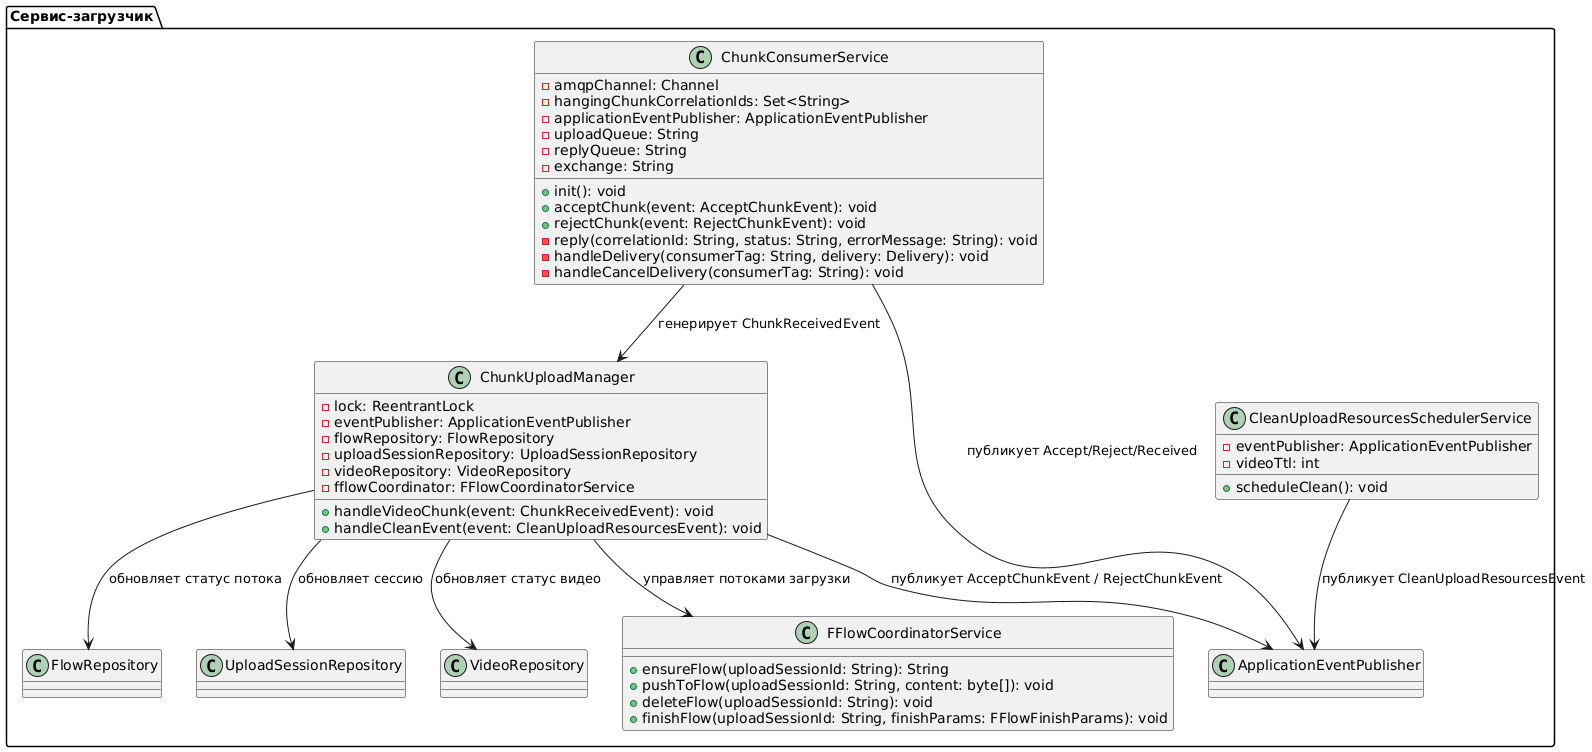
\includegraphics [scale=0.3] {my_folder/images//uml_uploader}
		\caption{UML-диаграмма сервиса-загрузчика} 
		\label{fig:uml_uploader}  
	\end{figure}
	
	\section{Разработка видеоплеера}

	Видеоплеер необходим для воспроизведения адаптивного потокового видеоконтента, представленного в нескольких синхронизированных потоках. Основная задача видеоплеера - обеспечить пользователям возможность удобного переключения между потоками и предоставить качественный просмотр видеоматериалов без задержек и ошибок вне зависимости от окружения. Для этого он и должен поддерживать работу с протоколами DASH и HLS. Как было отмечено ранее, клиентское приложение разделяется на три составляющих: компоненты интерфейса, хранилище данных и менеджеры событий. Рассмотрим их в отдельности.

	\subsection{Хранилище}

	Redux-хранилище является единственным источником истины для всех компонентов приложения. Это означает, что все необходимые данные компоненты интерфейса берут из хранилища с помощью хука useSelector. Поэтому все данные нельзя хранить в общей линейной структуре, они должны быть разделены на зоны ответственности. Видеоплеер содержит следующие основные состояния:

	\begin{itemize}[label=$\bullet$]
		\item player – отвечает за воспроизведение и содержит следующие подсостояния:
		\begin{itemize}[label=$\circ$]
			\item status – текущий статус проигрывания (PAUSED, PLAYING, FINISHED);
			\item currentTime и duration – текущее положение и длительность видео;
			\item isFullScreenOpened – полноэкранный режим;
			\item volume – уровень громкости;
			\item isMuted – включён ли режим "без звука".
		\end{itemize}
		Эти состояния распространяются на все проигрываемые потоки.
		\item video – управляет метаданными видео и потоками:
		\begin{itemize}[label=$\circ$]
			\item id, title, description, uploadedAt – общая информация о видео;
			\item flowById, flowIds, mainFlowId – список потоков и идентификатор текущего основного потока.
		\end{itemize}
		\item config – содержит настройки интерфейса, которые определяются с помощью переменных окружения:
		\begin{itemize}[label=$\circ$]
			\item isControlsHideable – может ли интерфейс управления автоматически скрываться.
		\end{itemize}
		\item error – отслеживает ошибки:
		\begin{itemize}[label=$\circ$]
			\item type – тип возникшей ошибки или null, если ошибка отсутствует.
		\end{itemize}
	\end{itemize}

	Хранилище предоставляет набор действий (action) для управления изменениями состояния. Эти события будут использоваться менеджером событий далее. Например, экшен setTime используется для синхронного обновления времени и длительности видео, а setStatus – для управления статусом воспроизведения.

	\subsection{Менеджер событий}

	Для обработки событий используется архитектурный паттерн саг, реализуемый Redux-Saga. Это означает, что у саг (обработчиков событий) есть древовидная структура. Корневая сага делегирует обработку дочерним. Саги используют класс VideoManager, который представляет динамический словарь, способный оповещать интерфейс об изменениях в его содержании. В качестве значений он содержит экземпляры браузерных плееров потоков. Рассмотрим каждую сагу в порядке очереди от корня к дочерним узлам ниже:
	
	\begin{itemize}[label=$\bullet$]
		\item fillContent – при инициализации получает ID видео из адресной строки, запрашивает данные о видео с сервера и проверяет статус. Если видео раздаётся (DISTRIBUTED), то заполняет хранилище метаданными (id, title, description, uploadedAt), списком потоков (flows) и устанавливает основной поток (mainFlowId). Если статус видео иной или потоки отсутствуют, выставляется соответствующая ошибка в хранилище;
		\item handleUpdateFlows – отслеживает событие updateFlows и создаёт экземпляры видеоплееров с помощью поддерживаемой в окружении технологии (DASH или HLS) для новых потоков, добавляя их в менеджер потоков;
		\item playSaga – запускает воспроизведение всех видеопотоков при срабатывании события play и устанавливает статус в PLAYING;
		\item pauseSaga – останавливает воспроизведение всех видеопотоков при срабатывании события pause и устанавливает статус в PAUSED;
		\item reloadSaga – перематывает видеопотоки на начало и запускает воспроизведение при экшене reload;
		\item seekSaga – перематывает видеопотоки на указанный временной промежуток при действии seek;
		\item togglePlaySaga – переключает воспроизведение в зависимости от текущего состояния (PLAYING, PAUSED, FINISHED) при действии togglePlay;
		\item toggleSoundSaga – включает или отключает звук при действии toggleSound;
		\item updateVolumeSaga – применяет новую громкость к главному потоку при действии setVolume;
		\item updateIsMutedSaga – устанавливает заглушение звука основного потока при действии setIsMuted;
		\item uploadMainFlowWatcher – отслеживает изменения основного потока (setMainFlowId), обновляет обработчики событий и состояние звука, отписываясь от старых и подписываясь на новые события потока.
	\end{itemize}

	\subsection{Компоненты интерфейса}
	
	Компоненты интерфейса содержат древовидную структуру с переиспользуемыми узлами для того, чтобы избежать повторения кода, а также выстраивать большое масштабируемое DOM дерево браузерной страницы. Рассмотрим каждый из компонентов в порядке очереди от корня к узлам ниже:
	
	\begin{itemize}[label=$\bullet$]
		\item App: корневой компонент, в котором собирается вся структура плеера. Он получает данные из хранилища (потоки, статус плеера, настройки) и отображает основной и второстепенные видеопотоки с помощью компонентов Slot. Компонент следит за движениями мыши, чтобы скрывать/показывать панель управления: используется состояние lastWasTouched, которое обновляется при событиях onClick и onMouseMove на контейнере main. Также реализована подписка на событие fullscreenchange через document.addEventListener, чтобы отслеживать вход и выход из полноэкранного режима. Обрабатывается завершение видео (PlayerStatus.FINISHED) и обновление текущего времени (setTime);
		\item Slot: отвечает за отображение одного видеопотока. Получает HTMLVideoElement из video-manager по flowId и встраивает его в DOM. При размонтировании удаляет видеоэлемент. Реализует переключение потока по клику с помощью передачи событий вверх по дереву;
		\item Controls: панель управления, отображаемая в нижней части плеера. В зависимости от статуса воспроизведения отображает разные состояния (play, pause, reload) и вызывает соответствующие экшены (play, pause, reload). Также содержит компоненты управления временем (TimeRange, TimeIndicator) и громкостью (VolumeControl). Обрабатывает нажатие кнопки полноэкранного режима;
		\item TimeRange: временная шкала. Рассчитывает прогресс воспроизведения и отрисовывает его с помощью Range. Обрабатывает движение мыши, клик и перемещение по шкале. Для этого подписывается на события mousemove и mouseup глобально через window.addEventListener, что позволяет точно отслеживать позицию мыши даже за пределами компонента. При отпускании мыши производится вызов экшена seek на рассчитанное время;
		\item TimeIndicator – отображает текущее время воспроизведения и общее время видео. Получает значения из хранилища (currentTime, duration) и преобразует их в форматированную строку, понятную пользователю;
		\item VolumeControl: отображает иконку звука в зависимости от уровня громкости или статуса isMuted. Использует Range для изменения громкости. Обрабатывает клики для включения/выключения звука и изменение громкости с помощью мыши. Использует события mousedown, mousemove, mouseup, а также mouseenter и mouseleave для управления состоянием регулировки звука. Вызывает экшен setVolume или toggleSound;
		\item Range: универсальный компонент шкалы прогресса. Используется в TimeRange и VolumeControl. Обрабатывает события мыши (enter, leave, down, move, up), рассчитывает прогресс по положению курсора и передаёт результат в родительский компонент через колбэки. Внутри компонента используется useLayoutEffect для подписки на глобальные события mousemove и mouseup с последующим удалением подписки при размонтировании.
	\end{itemize}

	UML-диаграмма компонентов интерфейса видеоплеера представлена на рисунке \ref{fig:uml_player}.

	\begin{figure}[ht!] 
		\center
		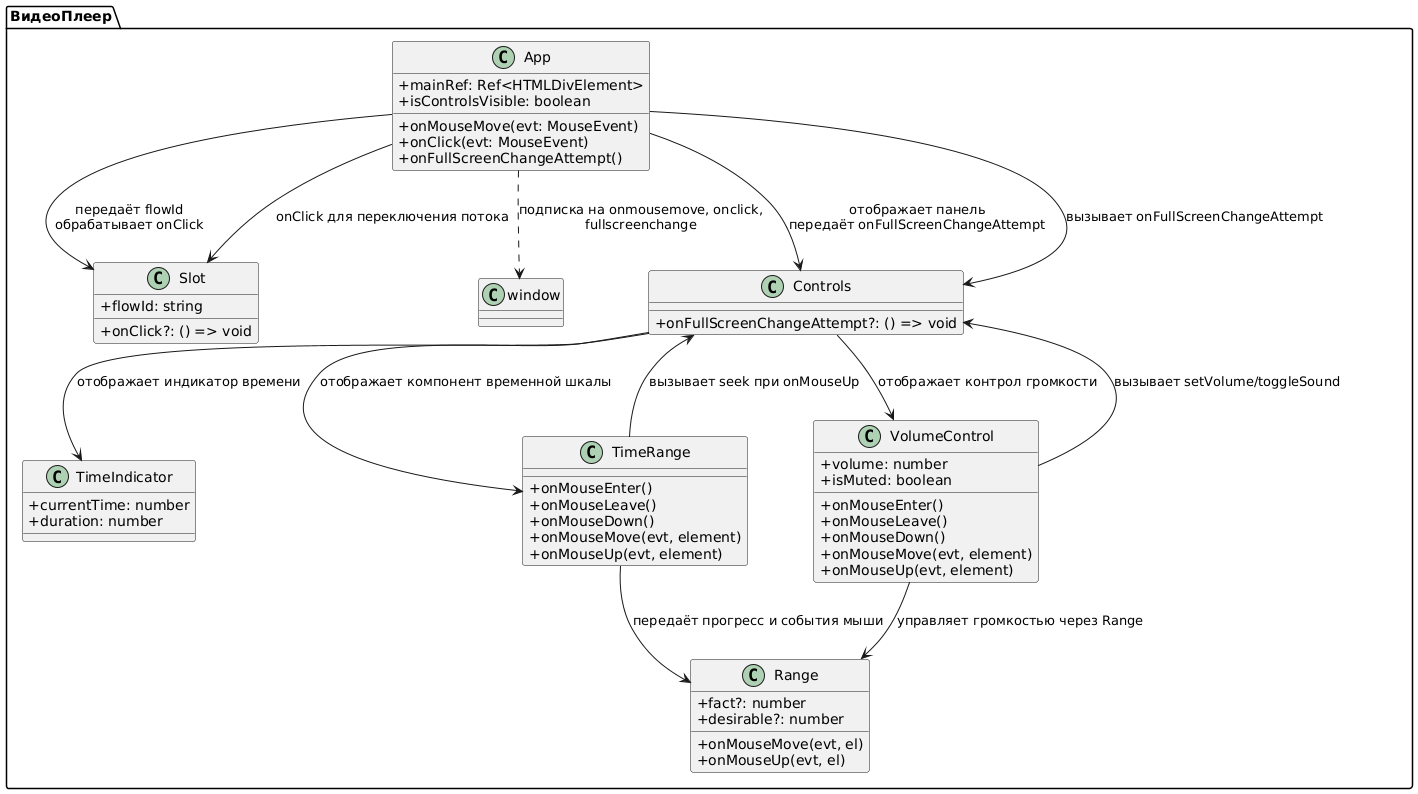
\includegraphics [scale=0.33] {my_folder/images//uml_player}
		\caption{UML-диаграмма компонентов интерфейса видеоплеера} 
		\label{fig:uml_player}  
	\end{figure}

	Интерфейс плеера представлен на рисунке \ref{fig:player_interface}.

	\begin{figure}[ht!] 
		\center
		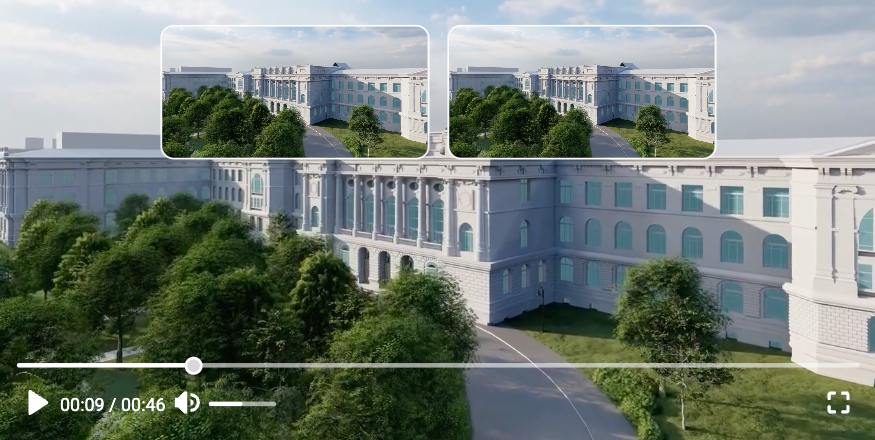
\includegraphics [scale=0.37] {my_folder/images//player_interface}
		\caption{Интерфейс видеоплеера} 
		\label{fig:player_interface}  
	\end{figure}

	\section{Разработка редактора синхронизации}
	
	Редактор синхронизации предназначен для локальной работы в браузере пользователя с потоками видео. Он должен содержать функциональность создания кандидатов на загрузку потоков видео, их удаления, изменения порядка, непосредственно загрузку, управления метаданными видео. Это клиентское приложение, как и видеоплеер, содержит большое количество событий и состояний, поэтому разделяется таким же образом на три составляющих: хранилище, менеджеры событий и компоненты интерфейса. Рассмотрим их ниже.
	
	\subsection{Хранилище}
	
	Хранилище представляет собой единый источник истины для всего приложения и структурировано по нескольким основным областям состояния, которые представлены ниже:
	
	\begin{itemize}[label=$\bullet$]
		\item \textbf{auth} – отвечает за аутентификацию пользователя и включает:
		\begin{itemize}[label=$\circ$]
			\item \textit{Состояния:}
			\begin{itemize}[label=--]
				\item accessToken — токен доступа пользователя;
				\item refreshToken — токен обновления пользователя.
			\end{itemize}
			\item \textit{События:}
			\begin{itemize}[label=--]
				\item login — осуществление аутентификации;
				\item logout — осуществление деаутентификации;
				\item register — регистрация пользователя;
				\item updateTokens — обновление токенов;
				\item reset — удаление токенов из хранилища.
			\end{itemize}
		\end{itemize}
		
		\item \textbf{stage} — текущее состояние экрана приложения:
		\begin{itemize}[label=$\circ$]
			\item SYNCHRONIZING — форма добавления потоков;
			\item LOADING — ожидание загрузки;
			\item UPLOADING — активная загрузка файлов;
			\item DISTRIBUTION — вывод итоговой ссылки.
		\end{itemize}
		
		\item \textbf{flowCandidates} — список временных идентификаторов потоков:
		\begin{itemize}[label=$\circ$]
			\item addCandidate — добавление кандидата;
			\item deleteCandidateById — удаление кандидата по идентификатору;
			\item addCandidateVideoAction — добавление кандидата с активным видео;
			\item deleteCandidateByIdAction — удаление кандидата с активным видео.
		\end{itemize}
		
		\item \textbf{upload} — информация о загружаемых потоках:
		\begin{itemize}[label=$\circ$]
			\item \textit{Состояния:}
			\begin{itemize}[label=--]
				\item flowIds — список идентификаторов потоков;
				\item flowById — словарь с метаданными и прогрессом;
				\item commonStatus — общее состояние процесса загрузки.
			\end{itemize}
			\item \textit{События:}
			\begin{itemize}[label=--]
				\item updateFlows — обновление текущих потоков;
				\item updateCommonStatus — обновление статуса загрузки.
			\end{itemize}
		\end{itemize}
		
		\item \textbf{distribution} — результат успешной загрузки:
		\begin{itemize}[label=$\circ$]
			\item playerUrl — URL плеера, сгенерированный после дистрибуции.
		\end{itemize}
	\end{itemize}

	\subsection{Менеджер событий}
	
	Для обработки асинхронных действий, как и в видеоплеере, используется архитектурный паттерн саг. И для того, чтобы контролировать жизненный цикл кандидатов потоков видео, также будет реализован класс VideoManager вместе с react-хуком useVideoManager, который будет обновлять состояние приложения при изменении потоков видео.

	Рассмотрим функциональность каждой из саг ниже:
	\begin{itemize}[label=$\bullet$]
		\item loginSaga — выполняет POST-запрос на /auth/login, получает токены и сохраняет их в localStorage. При успешном запросе обновляет состояние auth;
		\item logoutSaga — удаляет токены из localStorage и сбрасывает состояние auth;
		\item registerSaga — выполняет POST-запрос на регистрацию пользователя;
		\item addCandidateVideoSaga — добавляет Blob-видео в VideoManager по candidateId после выбора пользователем;
		\item deleteCandidateByIdSaga — удаляет поток из хранилища и удаляет соответствующее видео из VideoManager по идентификатору;
		\item startUploadSaga — главная сага загрузки, которая реализует следующую логику:
		\begin{itemize}[label=$\circ$]
			\item Переключает интерфейс в режим ожидания (LOADING);
			\item Получает список кандидатов и соответствующие видеофайлы из VideoManager;
			\item Отправляет метаданные на сервер (заголовок, описание, размеры файлов);
			\item Получает список потоков и обновляет хранилище;
			\item Копирует видеофайлы из кандидатов в основные потоки в VideoManager;
			\item Загружает видео по частям (вызов uploadFlowSaga);
			\item Параллельно запускает pollVideoState, отслеживающую статус загрузки;
			\item После окончания загрузки и распределения устанавливает URL плеера и переключает интерфейс на DISTRIBUTION. При ошибке возвращает SYNCHRONIZING.
		\end{itemize}
		\item uploadFlowSaga — вспомогательная сага, разбивающая видео на чанки и отправляющая их на сервер;
		\item pollVideoState — опрашивает состояние видео на сервере с интервалом STATE\_POLLING\_DELAY. При получении статуса BLOCKED или DISTRIBUTED завершает выполнение.
	\end{itemize}
	
	Общая UML-диаграмма компонентов хранилища и саг приложения представлена на рисунке \ref{fig:uml_sync_sagas_store}.
	
	\begin{figure}[ht!] 
		\center
		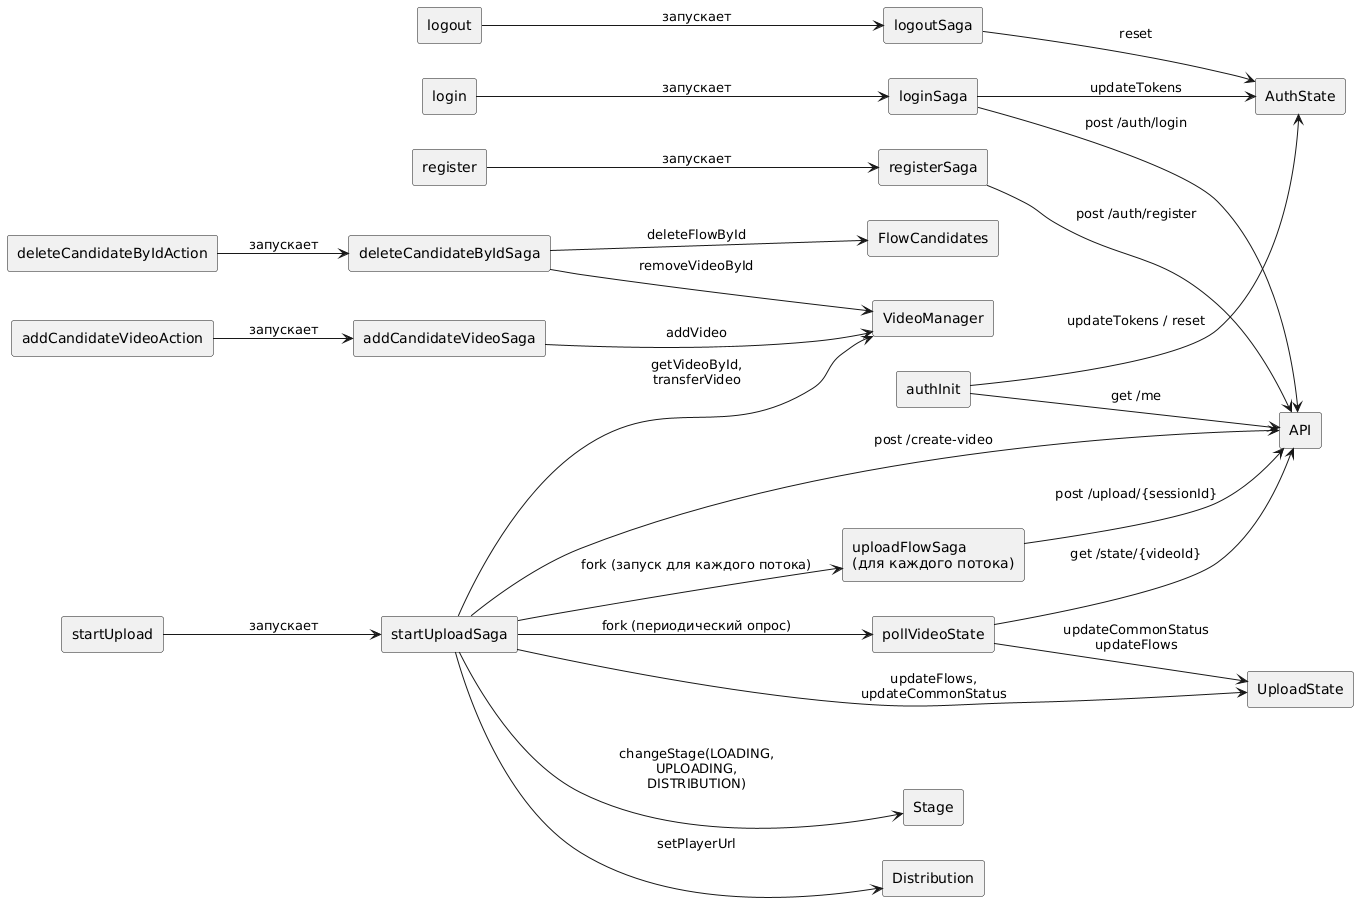
\includegraphics [scale=0.33] {my_folder/images//uml_sync_sagas_store}
		\caption{UML-диаграмма компонентов хранилища и саг редактора синхронизации} 
		\label{fig:uml_sync_sagas_store}  
	\end{figure}
	